\documentclass[11pt]{article}
\usepackage{amssymb}
\usepackage{amsmath}
\usepackage{tikz}
\usetikzlibrary{arrows.meta}
\usepackage{array,colortbl,xcolor}

\newcommand{\T}{\mathrm{T}}

\begin{document}

    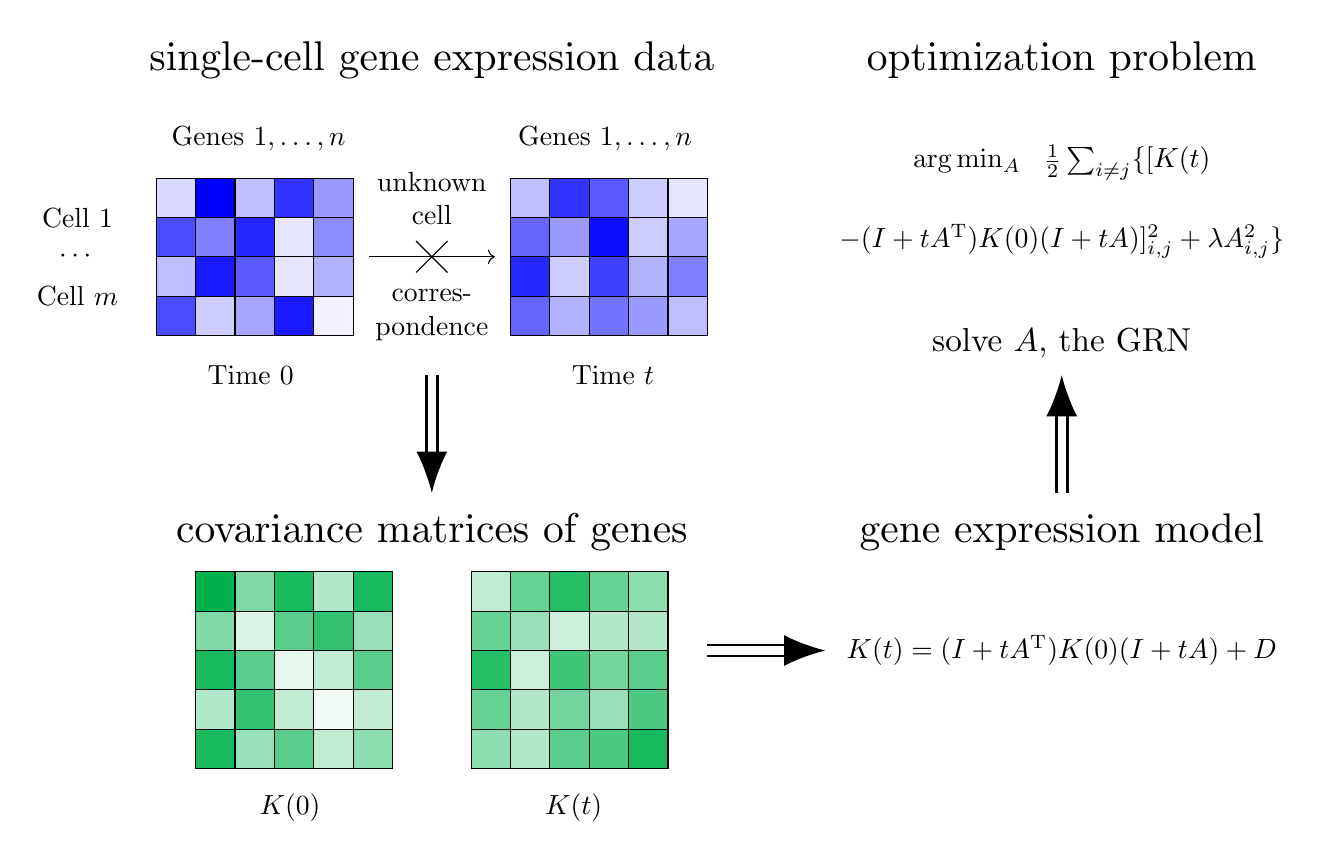
\begin{tikzpicture}
   \draw[black] (-9.5,0) rectangle (-7,2); 
   \draw[black] (-5,0) rectangle (-2.5,2); 
    \draw[->]        (-6.8,1)   -- (-5.2,1);
    \draw       (-6.2,1.2)   -- (-5.8,0.8);
    \draw       (-6.2,0.8)   -- (-5.8,1.2);
    \filldraw[fill=blue!70] (-9.5,0) rectangle (-9,0.5);
    \filldraw[fill=blue!20] (-9,0) rectangle (-8.5,0.5);
    \filldraw[fill=blue!35] (-8.5,0) rectangle (-8,0.5);
    \filldraw[fill=blue!90] (-8,0) rectangle (-7.5,0.5);
    \filldraw[fill=blue!5] (-7.5,0) rectangle (-7,0.5);
    \filldraw[fill=blue!25] (-9.5,0.5) rectangle (-9,1);
    \filldraw[fill=blue!90] (-9,0.5) rectangle (-8.5,1);
    \filldraw[fill=blue!65] (-8.5,0.5) rectangle (-8,1);
    \filldraw[fill=blue!10] (-8,0.5) rectangle (-7.5,1);
    \filldraw[fill=blue!30] (-7.5,0.5) rectangle (-7,1);
    \filldraw[fill=blue!70] (-9.5,1) rectangle (-9,1.5);
    \filldraw[fill=blue!50] (-9,1) rectangle (-8.5,1.5);
    \filldraw[fill=blue!85] (-8.5,1) rectangle (-8,1.5);
    \filldraw[fill=blue!10] (-8,1) rectangle (-7.5,1.5);
    \filldraw[fill=blue!45] (-7.5,1) rectangle (-7,1.5);
    \filldraw[fill=blue!15] (-9.5,1.5) rectangle (-9,2);
    \filldraw[fill=blue!100] (-9,1.5) rectangle (-8.5,2);
    \filldraw[fill=blue!25] (-8.5,1.5) rectangle (-8,2);
    \filldraw[fill=blue!80] (-8,1.5) rectangle (-7.5,2);
    \filldraw[fill=blue!40] (-7.5,1.5) rectangle (-7,2);
    \filldraw[fill=blue!60] (-5,0) rectangle (-4.5,0.5);
    \filldraw[fill=blue!30] (-4.5,0) rectangle (-4,0.5);
    \filldraw[fill=blue!55] (-4,0) rectangle (-3.5,0.5);
    \filldraw[fill=blue!40] (-3.5,0) rectangle (-3,0.5);
    \filldraw[fill=blue!25] (-3,0) rectangle (-2.5,0.5);
    \filldraw[fill=blue!85] (-5,0.5) rectangle (-4.5,1);
    \filldraw[fill=blue!20] (-4.5,0.5) rectangle (-4,1);
    \filldraw[fill=blue!75] (-4,0.5) rectangle (-3.5,1);
    \filldraw[fill=blue!30] (-3.5,0.5) rectangle (-3,1);
    \filldraw[fill=blue!50] (-3,0.5) rectangle (-2.5,1);
    \filldraw[fill=blue!60] (-5,1) rectangle (-4.5,1.5);
    \filldraw[fill=blue!40] (-4.5,1) rectangle (-4,1.5);
    \filldraw[fill=blue!95] (-4,1) rectangle (-3.5,1.5);
    \filldraw[fill=blue!20] (-3.5,1) rectangle (-3,1.5);
    \filldraw[fill=blue!35] (-3,1) rectangle (-2.5,1.5);
    \filldraw[fill=blue!25] (-5,1.5) rectangle (-4.5,2);
    \filldraw[fill=blue!80] (-4.5,1.5) rectangle (-4,2);
    \filldraw[fill=blue!65] (-4,1.5) rectangle (-3.5,2);
    \filldraw[fill=blue!20] (-3.5,1.5) rectangle (-3,2);
    \filldraw[fill=blue!10] (-3,1.5) rectangle (-2.5,2);
\node[scale=1.5] at (-6,3.5) {single-cell gene expression data};
\node at (-10.5,1.5) {Cell 1};
\node at (-6,1.7) {{\begin{tabular}{c} unknown \\ cell \end{tabular}}};
\node at (-6,0.3) {{\begin{tabular}{c} corres- \\ pondence \end{tabular}}};
\node at (-10.5,0.5) {Cell $m$};
\node at (-10.5,1) {$\cdots$};
\node at (-8.2,2.5) {Genes $1,\ldots,n$};
\node at (-3.8,2.5) {Genes $1,\ldots,n$};
\node at (-8.3,-0.5) {Time $0$};
\node at (-3.7,-0.5) {Time $t$};
\draw [line width=1pt, double distance=3pt,
             arrows = {-Latex[length=0pt 3 0]}]        (-6,-0.5)   -- (-6,-2);
\draw[black] (-9,-5) rectangle (-7,-3); 
\draw[black] (-5,-5) rectangle (-3,-3); 
\node[scale=1.5] at (-6,-2.5) {covariance matrices of genes};
    \filldraw[fill=blue!30!green!30] (-9,-5) rectangle (-8.5,-4.5);
    \filldraw[fill=blue!30!green!80] (-8.5,-5) rectangle (-8,-4.5);
    \filldraw[fill=blue!30!green!25] (-8,-5) rectangle (-7.5,-4.5);
    \filldraw[fill=blue!30!green!5] (-7.5,-5) rectangle (-7,-4.5);
    \filldraw[fill=blue!30!green!25] (-7,-5) rectangle (-6.5,-4.5);

    \filldraw[fill=blue!30!green!90] (-9,-4.5) rectangle (-8.5,-4);
    \filldraw[fill=blue!30!green!65] (-8.5,-4.5) rectangle (-8,-4);
    \filldraw[fill=blue!30!green!10] (-8,-4.5) rectangle (-7.5,-4);
    \filldraw[fill=blue!30!green!25] (-7.5,-4.5) rectangle (-7,-4);
    \filldraw[fill=blue!30!green!65] (-7,-4.5) rectangle (-6.5,-4);

    \filldraw[fill=blue!30!green!50] (-9,-4) rectangle (-8.5,-3.5);
    \filldraw[fill=blue!30!green!15] (-8.5,-4) rectangle (-8,-3.5);
    \filldraw[fill=blue!30!green!65] (-8,-4) rectangle (-7.5,-3.5);
    \filldraw[fill=blue!30!green!80] (-7.5,-4) rectangle (-7,-3.5);
    \filldraw[fill=blue!30!green!40] (-7,-4) rectangle (-6.5,-3.5);

    \filldraw[fill=blue!30!green!100] (-9,-3.5) rectangle (-8.5,-3);
    \filldraw[fill=blue!30!green!50] (-8.5,-3.5) rectangle (-8,-3);
    \filldraw[fill=blue!30!green!90] (-8,-3.5) rectangle (-7.5,-3);
    \filldraw[fill=blue!30!green!30] (-7.5,-3.5) rectangle (-7,-3);    
    \filldraw[fill=blue!30!green!90] (-7,-3.5) rectangle (-6.5,-3);

    \filldraw[fill=blue!30!green!90] (-9,-5.5) rectangle (-8.5,-5);
    \filldraw[fill=blue!30!green!40] (-8.5,-5.5) rectangle (-8,-5);
    \filldraw[fill=blue!30!green!65] (-8,-5.5) rectangle (-7.5,-5);
    \filldraw[fill=blue!30!green!25] (-7.5,-5.5) rectangle (-7,-5);
    \filldraw[fill=blue!30!green!45] (-7,-5.5) rectangle (-6.5,-5);


    \filldraw[fill=blue!30!green!60] (-5.5,-5) rectangle (-5,-4.5);
    \filldraw[fill=blue!30!green!30] (-5,-5) rectangle (-4.5,-4.5);
    \filldraw[fill=blue!30!green!55] (-4.5,-5) rectangle (-4,-4.5);
    \filldraw[fill=blue!30!green!40] (-4,-5) rectangle (-3.5,-4.5);    
    \filldraw[fill=blue!30!green!70] (-3.5,-5) rectangle (-3,-4.5); 
    \filldraw[fill=blue!30!green!85] (-5.5,-4.5) rectangle (-5,-4);
    \filldraw[fill=blue!30!green!20] (-5,-4.5) rectangle (-4.5,-4);
    \filldraw[fill=blue!30!green!75] (-4.5,-4.5) rectangle (-4,-4);
    \filldraw[fill=blue!30!green!55] (-4,-4.5) rectangle (-3.5,-4); 
    \filldraw[fill=blue!30!green!65] (-3.5,-4.5) rectangle (-3,-4); 
    \filldraw[fill=blue!30!green!60] (-5.5,-4) rectangle (-5,-3.5);
    \filldraw[fill=blue!30!green!40] (-5,-4) rectangle (-4.5,-3.5);
    \filldraw[fill=blue!30!green!20] (-4.5,-4) rectangle (-4,-3.5);
    \filldraw[fill=blue!30!green!30] (-4,-4) rectangle (-3.5,-3.5); 

    \filldraw[fill=blue!30!green!30] (-3.5,-4) rectangle (-3,-3.5); 
    \filldraw[fill=blue!30!green!25] (-5.5,-3.5) rectangle (-5,-3);
    \filldraw[fill=blue!30!green!60] (-5,-3.5) rectangle (-4.5,-3);
    \filldraw[fill=blue!30!green!85] (-4.5,-3.5) rectangle (-4,-3);
    \filldraw[fill=blue!30!green!60] (-4,-3.5) rectangle (-3.5,-3);
    \filldraw[fill=blue!30!green!45] (-3.5,-3.5) rectangle (-3,-3);

    \filldraw[fill=blue!30!green!45] (-5.5,-5.5) rectangle (-5,-5);
    \filldraw[fill=blue!30!green!30] (-5,-5.5) rectangle (-4.5,-5);
    \filldraw[fill=blue!30!green!65] (-4.5,-5.5) rectangle (-4,-5);
    \filldraw[fill=blue!30!green!70] (-4,-5.5) rectangle (-3.5,-5);
    \filldraw[fill=blue!30!green!90] (-3.5,-5.5) rectangle (-3,-5);
\node at (-7.8,-6) {$K(0)$};
\node at (-4.2,-6) {$K(t)$};
\draw [line width=1pt, double distance=3pt,
             arrows = {-Latex[length=0pt 3 0]}]        (-2.5,-4)   -- (-1,-4);
\draw [line width=1pt, double distance=3pt,
             arrows = {-Latex[length=0pt 3 0]}]        (2,-2)   -- (2,-0.5);
\node[scale=1.5] at (2,-2.5) {gene expression model};
\node at (2,-4) {$K(t)=(I+tA^\T)K(0)(I+tA)+D$};
\node[scale=1.5] at (2,3.5) {optimization problem};
\node at (2,2.2) {$\arg\min_{A}\ \ \frac{1}{2}\sum_{i\ne j} \{[K(t)$};
\node at (2,1.2) {$-(I+tA^\T)K(0)(I+tA)]^2_{i,j}+\lambda A^2_{i,j}\}$};
\node[scale=1.2] at (2,-0.1) {solve $A$, the GRN};
\end{tikzpicture}

\end{document}